% Created 2014-12-02 Tue 16:56
\documentclass[11pt]{article}
\usepackage[utf8]{inputenc}
\usepackage[french]{babel}
\usepackage[T1]{fontenc}
\usepackage{fixltx2e}
\usepackage{graphicx}
\usepackage{longtable}
\usepackage{array}
\usepackage{float}
\usepackage{wrapfig}
\usepackage{rotating}
\usepackage[normalem]{ulem}
\usepackage{amsmath}
\usepackage{textcomp}
\usepackage{marvosym}
\usepackage{wasysym}
\usepackage{amssymb}
\usepackage{hyperref}
\usepackage[a4paper, margin=1cm]{geometry}
\author{Corentin Cadiou, Aymeric Fromherz, Lucas Verney}
\date{\today}
\title{Système digital, rapport de projet}
\begin{document}

\maketitle
\section*{Introduction}
Pour divers projets électroniques personnels, nous utilisons régulièrement des micro-contrôleurs 8 bits vendus par la marque \emph{Atmel} et utilisant une architecture et l'\emph{instruction set} AVR\footnote{\url{http://people.ece.cornell.edu/land/courses/ece4760/AtmelStuff/AVRinstr2002.PDF}}, notamment ceux vendus avec des cartes de développement ``Arduino''. Dans le cadre du projet du cours de ``Système digital'', nous avons décidé de simuler un tel micro-contrôleur, plutôt qu'un processeur MIPS standard.

Il existe une très grande variété de micro-contrôleurs de ce type, et afin de réduire la complexité du projet, nous avons décidé de nous concentrer sur un ATTiny4\footnote{\url{http://www.atmel.com/images/atmel-8127-avr-8-bit-microcontroller-attiny4-attiny5-attiny9-attiny10_datasheet.pdf}}, qui supporte un jeu de 54 instructions, possède 16 registres 8 bits, 512 octets de ROM et 32 octets de RAM. C'est le modèle de ce type le plus simple que nous ayons trouvé, et les modéles supérieurs n'apportent que peu de nouvelles fonctionnalités intéressantes pour cette simulation : \emph{ADC} (\emph{Analog Digital Converter}), \dots.

\section{Architecture}
Les microcontrolleurs ATTiny4 sont des microcontrolleurs 8bits avec un
jeu de 54 instructions pour 16 registres 8bits, \emph{little-endian}, qui
fonctionnent généralement à une dizaine de $MHz$. Ils possèdent en
outre 512 octets de ROM et 32 octets de RAM. En plus des 16 registres
généraux, les ATTiny4 possèdent d'autres registres utiles à implémenter pour :
\begin{itemize}
  \item les \emph{input/output}(I/O) ;
  \item un registre de statut (voir
    Section~\ref{sec:registre-de-statut}) stockant par exemple les
    retenues ;
  \item un pointeur de pile ;
  \item un compteur d'instruction (sur 9 bits) ;
  \item un registre d'instruction (sur 16 bits) ;
\end{itemize}
%todo: image
Ces microcontrolleurs possèdent un oscillateur interne leur servant de
référence temporelle pour leur \emph{timer}.
\subsection{Registres}\label{sec:registres}
Il y a 16 registres 8 bits, numérotés de \verb|R16| à \verb|R31|. Les
six derniers (\verb|R26|-\verb|R31|) peuvent être utilisé pour faire
de l'adressage indirect de la mémoire sur 16 bits grâce à 3 meta-registres \verb|X|, \verb|Y|
et \verb|Z|. Se référer au tableau~\ref{tab:meta-registres}.
\begin{table}[htbp]
  \centering
  \begin{tabular}{|c|c|c|}
\hline
    Registre & Bits de poids fort & Bits de poids faible \\
\hline
\hline
    \verb|X| & \verb|R27| & \verb|R26| \\
\hline
    \verb|Y| & \verb|R29| & \verb|R28| \\
\hline
    \verb|Z| & \verb|R31| & \verb|R30| \\
\hline
  \end{tabular}
  \caption{\label{tab:meta-registres}Composition des meta-registres
    $\texttt{X}$, $\texttt{Y}$ et $\texttt{Z}$.}

\end{table}

Le registre de statut contient 8 bits de \emph{flag} (voir
tableau~\ref{tab:status_register}).
\begin{table}[h!tbp]
  \centering
  \begin{tabular}{c c m{30em}}
    Bit & \emph{flag} & Désignation \\
\hline
    0 & \texttt{C} & \emph{carry flag} : retenue \\
    1 & \texttt{Z} & \emph{zero flag} : résultat nul \\
    2 & \texttt{N} & \emph{negative flag} : résultat négatif \\
    3 & \texttt{V} & \emph{two's complement overflow flag} : dépassement pour
            le complément à deux \\
    4 & \texttt{S} & \emph{sign bit} : $\mathtt{S} = \mathtt{N} \oplus
            \mathtt{V}$ \\
    5 & \texttt{H} & \emph{half carry flag} \\
    6 & \texttt{T} & \emph{bit copy storage} : les instructions de copie de bit
            \texttt{BLD} et \texttt{BDT} utilisent ce bit comme source
            ou destination pour le bit modifié \\
    7 & \texttt{I} & \emph{global interrupt enabled} : contrôle l'activation
            des \emph{interrupt}s.
  \end{tabular}
  \caption{\label{tab:status_register}Signification des bits du registre de statut.}
\end{table}
\subsection{Mémoire}\label{sec:memoire}
L'ATTiny4 contient 512 octets de ROM. Le compteur d'instruction
ayant 9 bits, il est bien capable d'adresser les 256
emplacements mémoire en commencant à \texttt{0x000}. 
% todo : WTF magistral

Les emplacements mapés en mémoire incluent les I/O, la RAM et la
ROM. Le détail est donné dans le tableau
\begin{table}[htbp]
  \centering
  \begin{tabular}{|c|l|}
\hline
    \texttt{0x0000}…\texttt{0x003F} & I/O \\
\hline
    \texttt{0x0040}…\texttt{0x005F} & RAM \\
\hline
    \texttt{0x0060}…\texttt{0x3FFF} & Autre \\
\hline
    \texttt{0x4000}…\texttt{0x41FF} & ROM \\
\hline
    \texttt{0x4400}…\texttt{0xFFFF} & Autre \\
\hline
  \end{tabular}
  \caption{Carte de la mémoire.}
  \label{tab:memory-map}
\end{table}

\section{\emph{Instruction set}}
\subsection{Structure}
Chaque instruction est codée sur 16 bits et peuvent groupés par
instructions arithmétiques, logiques, de branchement, de chargement,
de \emph{flag} et autres. Chacune des instructions peut altérer des
bits dans le registre de statut.
\subsection{Modes d'adressage}
Les instructions peuvent utiliser l'adressage suivant :
\begin{itemize}
  \item Adressage direct d'un seul registre ;
   \begin{center}
     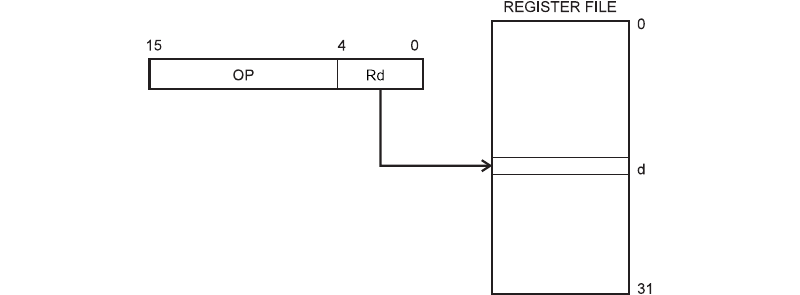
\includegraphics[width=0.5\textwidth]{images/direct_adressing.png}
   \end{center}
 \item Adressage direct de deux registres ;
   \begin{center}
     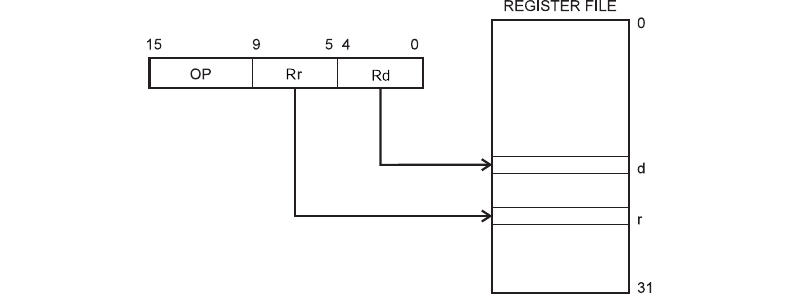
\includegraphics[width=0.5\textwidth]{images/direct_adressing_double.png}
   \end{center}
  \item Adressage direct d'I/O ;
   \begin{center}
     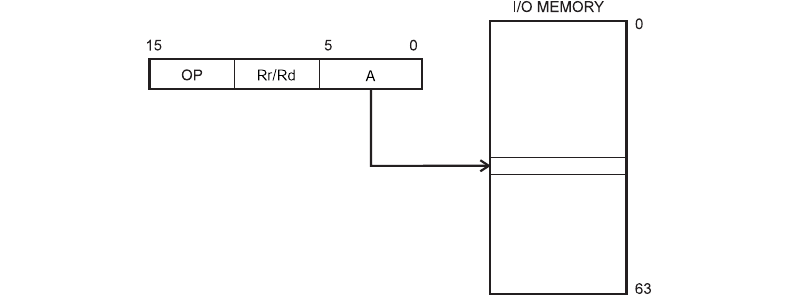
\includegraphics[width=0.5\textwidth]{images/direct_adressing_IO.png}
   \end{center}
  \item Adressage indirect grâce aux registres \texttt{X}, \texttt{Y}
    ou \texttt{Z} ;
   \begin{center}
     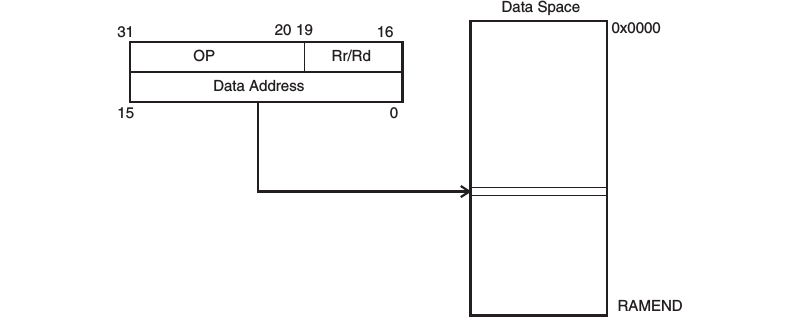
\includegraphics[width=0.5\textwidth]{images/direct_data_adressing.png}
   \end{center}
  \item Adressage indirect grâce aux registres \texttt{X}, \texttt{Y}
    ou \texttt{Z} avec déplacement ;
   \begin{center}
     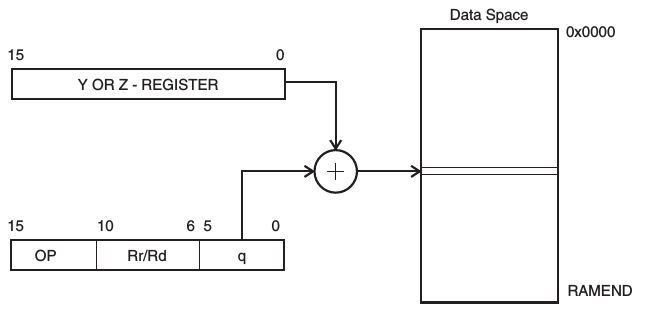
\includegraphics[width=0.5\textwidth]{images/data_indirect_displacement.png}
   \end{center}
  \item Adressage indirect grâce aux registres \texttt{X}, \texttt{Y}
    ou \texttt{Z} avec pré-incrémentation ;
   \begin{center}
     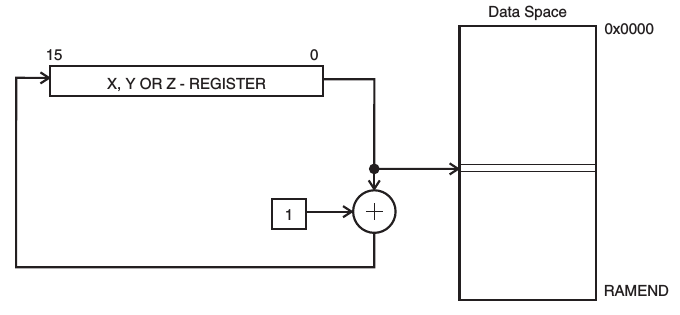
\includegraphics[width=0.5\textwidth]{images/data_indirect_postincrement.png}
   \end{center}
  \item Adressage indirect grâce aux registres \texttt{X}, \texttt{Y}
    ou \texttt{Z} avec post-incrémentation ;
   \begin{center}
     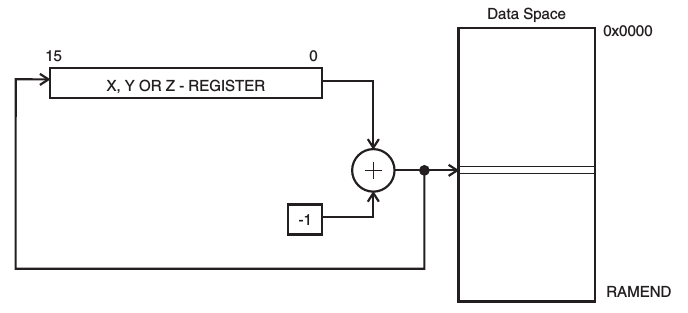
\includegraphics[width=0.5\textwidth]{images/data_indirect_predecrement.png}
   \end{center}
\end{itemize}
\subsection{\emph{Instruction set} complet}
\tiny
\noindent\begin{center}
    \begin{longtable}{|c|m{12em}|c|c|c|c|c|}
\hline
Mnemo. & Operation & Description & \#Clocks & PC & Flags & Opcode\\
\hline\hline
\endhead

\hline\hline
Mnemo. & Operation & Description & \#Clocks & PC & Flags & Opcode\\
\hline
\endfoot

\multicolumn{7}{|c|}{Arithmetic} \\\hline
ADD & $R_d \leftarrow R_d + R_r$ & Add without carry & 1 & 1 & $Z, C, N, V, S, H$ & \texttt{0000 11rd dddd rrrr}\\
ADC & $R_d \leftarrow R_d + R_r + C$ & Add with carry & 1 & 1 & $Z, C, N, V, S, H$ & \texttt{0001 11rd dddd rrrr}\\
SUB & $R_d \leftarrow R_d - R_r$ & Subtract without carry & 1 & 1 & $Z, C, N, V, S, H$ & \texttt{0001 10rd dddd rrrr}\\
SUBI & $R_d \leftarrow R_d - K$ & Subtract immediate & 1 & 1 & $Z, C, N, V, S, H$ & \texttt{0101 KKKK dddd KKKK}\\
SBC & $R_d \leftarrow R_d - R_r - C$ & Subtract with carry & 1 & 1 & $Z, C, N, V, S, H$ & \texttt{0000 10rd dddd rrrr}\\
SBCI & $R_d \leftarrow R_d - K - C$ & Subtract immediate with carry & 1 & 1 & $Z, C, N, V, S, H$ & \texttt{0100 KKKK dddd KKKK}\\
AND & $R_d \leftarrow R_d \text{ \& } R_r$ & Logical AND & 1 & 1 & $Z, N, V, S$ & \texttt{0010 00rd dddd rrrr}\\
ANDI & $R_d \leftarrow R_d \text{ \& } K$ & Logical AND with immediate & 1 & 1 & $Z, N, V, S$ & \texttt{0111 KKKK dddd KKKK}\\
OR & $R_d \leftarrow R_d \text{ | } R_r$ & Logical OR & 1 & 1 & $Z, N, V, S$ & \texttt{0010 10rd dddd rrrr}\\
ORI & $R_d \leftarrow R_d \text{ | } K$ & Logical OR with immediate & 1 & 1 & $Z, N, V, S$ & \texttt{0110 KKKK dddd KKKK}\\
EOR & $R_d \leftarrow R_d \text{ xor } R_r$ & Exclusive OR & 1 & 1 & $Z, N, V, S$ & \texttt{0010 01rd dddd rrrr}\\
COM & $R_d \leftarrow 0xFF - R_d$ & One's complement & 1 & 1 & $Z, C, N, V, S$ & \texttt{1001 010d dddd 0000}\\
NEG & $R_d \leftarrow 0x00 - R_d$ & Two's complement & 1 & 1 & $Z, C, N, V, S$, H & \texttt{1001 010d dddd 0001}\\
SBR & $R_d \leftarrow R_d \text{ | } K$ & Set bits in register & 1 & 1 & $Z, N, V, S$ & \texttt{0110 KKKK dddd KKKK}\\
CBR & $R_d \leftarrow R_d \text{ \& } (0xFFh - K)$ & Clear bits in register & 1 & 1 & $Z, N, V, S$ & \texttt{0111 }$\overline{\texttt{KKKK}}$\texttt{ dddd }$\mathtt{\overline{KKKK}}$\\ % TODO
INC & $R_d \leftarrow R_d + 1$ & Increment & 1 & 1 & $Z, N, V, S$ & \texttt{1001 010d dddd 0011}\\
DEC & $R_d \leftarrow R_d - 1$ & Decrement & 1 & 1 & $Z, N, V, S$ & \texttt{1001 010d dddd 1010}\\
TST & $R_d \leftarrow R_d \text{ \& } R_d$ & Test for zero or minus & 1 & 1 & $Z, N, V, S$ & \texttt{0010 00dd dddd dddd}\\
CLR & $R_d \leftarrow R_d \text{ xor } R_d$ & Clear register & 1 & 1 & $Z, N, V, S$ & \texttt{0010 01dd dddd dddd}\\
SER & $R_d \leftarrow 0xFF$ & Set all bits in register & 1 & 1 & None & \texttt{1110 1111 dddd 1111}\\
\hline\hline
\multicolumn{7}{|c|}{Branching} \\
\hline
RJMP & $PC \leftarrow PC + k + 1, STACK \leftarrow PC + 1, SP \leftarrow SP - 2$ & Relative jump & 2 & $k + 1$ & None & \texttt{1100 kkkk kkkk kkkk}\\
IJMP & $PC(15:0) \leftarrow Z, PC(21:16) \leftarrow 0$ & Indirect jump to $(Z)$ & 2 & See operation & None & \texttt{1001 0100 0000 1001}\\
RCALL & $PC \leftarrow PC + k + 1, STACK \leftarrow PC + 1, SP \leftarrow SP - 2$ & Relative subroutine call & 3 & $k + 1$ & None & \texttt{1101 kkkk kkkk kkkk}\\
ICALL & $PC(15:0) \leftarrow Z, PC(21:16) \leftarrow 0, STACK \leftarrow PC + 1, SP \leftarrow SP - 2$ & Indirect call to $(Z)$ & 3 & See operation & None & \texttt{1001 0101 0000 1001}\\
RET & $PC \leftarrow STACK, SP \leftarrow SP + 2$ & Subroutine return & 4 & See operation & None & \texttt{1001 0101 0000 1000}\\
RETI & $PC \leftarrow STACK, SP \leftarrow SP + 2$ & Interrupt return & 4 & See operation & $I$ & \texttt{1001 0101 0001 1000}\\
CPSE & $if(R_d = R_r) PC \leftarrow PC + 2 \text{ or } 3$ & Compare, skip if equal & 1 (false) / 2 (true) & 1 (false) / 2 (true) & None & \texttt{0001 00rd dddd rrrr}\\
CP & $R_d - R_r$ & Compare & 1 & 1 & $Z, C, N, V, S, H$ & \texttt{0001 01rd dddd rrrr}\\
CPC & $ R_d - R_r - C$ & Compare with carry & 1 & 1 & $Z, C, N, V, S, H$ & \texttt{0000 01rd dddd rrrr}\\
CPI & $R_d - K$ & Compare with immediate & 1 & 1 & $Z, C, N, V, S, H$ & \texttt{0011 KKKK dddd KKKK}\\
SBRC & $if(R_r(b) = 0) PC \leftarrow PC + 2 \text{ or } 3$ & Skip if bit in register cleared & 1 (false) / 2 (true) & 1 (false) / 2 (true) & None & \texttt{1111 110r rrrr 0bbb}\\
SBRS & $if(R_r(b) = 1) PC \leftarrow PC + 2 \text{ or } 3$ & Skip if bit in register set & 1 (false) / 2 (true) & 1 (false) / 2 (true) & None & \texttt{1111 110r rrrr 0bbb}\\
SBIC & $if(I/O(A, b) = 0) PC \leftarrow PC + 2 \text{ or } 3$ & Skip if bit in $I/O$ register cleared & 1 (false) / 2 (true) & 1 (false) / 2 (true) & None & \texttt{1001 1001 AAAA Abbb}\\
SBIS & $if(I/O(A, b) = 1) PC \leftarrow PC +2 \text{ or } 3$ & Skip if bit in $I/O$ register set & 1 (false) / 2 (true) & 1 (false) / 2 (true) & None & \texttt{1001 1011 AAAA Abbb}\\
BRBS & $if(SREG(s) = 1) PC \leftarrow PC + k + 1$ & Branch if status flag set & 1 (false) / 2 (true) & 1 (false) / $k + 1$ (true) & None & \texttt{1111 00kk kkkk ksss}\\
BRBC & $if(SREG(s) = 0) PC \leftarrow PC + k + 1$ & Branch if status flag cleared & 1 (false) / 2 (true) & 1 (false) / $k+1$ (true) & None & \texttt{1111 01kk kkkk ksss}\\
BREQ & $if(Z = 1) PC \leftarrow PC + k + 1$ & Branch if equal & 1 (false) / 2 (true) & 1 (false) / $k+1$ (true) & None & \texttt{1111 00kk kkkk k001}\\
BRNE & $if(Z = 0) PC \leftarrow PC + k + 1$ & Branch if not equal & 1 (false) / 2 (true) & 1 (false) / $k+1$ (true) & None & \texttt{1111 01kk kkkk k001}\\
BRCS & $if(C = 1) PC \leftarrow PC + k + 1$ & Branch if carry set & 1 (false) / 2 (true) & 1 (false) / $k+1$ (true) & None & \texttt{1111 00kk kkkk k000}\\
BRCC & $if(C = 0) PC \leftarrow PC + k + 1$ & Branch if carry cleared & 1 (false) / 2 (true) & 1 (false) / $k+1$ (true) & None & \texttt{1111 01kk kkkk k000}\\
BRSH & $if(C = 0) PC \leftarrow PC + k + 1$ & Branch if same or higher & 1 (false) / 2 (true) & 1 (false) / $k+1$ (true) & None & \texttt{1111 01kk kkkk k000}\\
BRLO & $if(C = 1) PC \leftarrow PC + k + 1$ & Branch if lower & 1 (false) / 2 (true) & 1 (false) / $k+1$ (true) & None & \texttt{1111 00kk kkkk k000}\\
BRMI & $if(N = 1) PC \leftarrow PC + k + 1$ & Branch if minus & 1 (false) / 2 (true) & 1 (false) / $k+1$ (true) & None & \texttt{1111 00kk kkkk k010}\\
BRPL & $if(N = 0) PC \leftarrow PC + k + 1$ & Branch if plus & 1 (false) / 2 (true) & 1 (false) / $k+1$ (true) & None & \texttt{1111 01kk kkkk k010}\\
BRGE & $if(N \text{ xor } V = 0) PC \leftarrow PC + k + 1$ & Branch if greater or equal, signed & 1 (false) / 2 (true) & 1 (false) / $k+1$ (true) & None & \texttt{1111 01kk kkkk k100}\\
BRLT & $if(N \text{ xor } V = 1) PC \leftarrow PC + k + 1$ & Branch if less than zero, signed & 1 (false) / 2 (true) & 1 (false) / $k+1$ (true) & None & \texttt{1111 00kk kkkk k100}\\
BRHS & $if(H = 1) PC \leftarrow PC + k + 1$ & Branch if half carry flag set & 1 (false) / 2 (true) & 1 (false) / $k+1$ (true) & None & \texttt{1111 00kk kkkk k101}\\
BRHC & $if(H = 0) PC \leftarrow PC + k + 1$ & Branch if half carry flag cleared & 1 (false) / 2 (true) & 1 (false) / $k+1$ (true) & None & \texttt{1111 01kk kkkk k101}\\
BRTS & $if(T = 1) PC \leftarrow PC + k + 1$ & Branch if $T$ flag set & 1 (false) / 2 (true) & 1 (false) / $k+1$ (true) & None & \texttt{1111 00kk kkkk k110}\\
BRTC & $if(T = 0) PC \leftarrow PC + k + 1$ & Branch if $T$ flag cleared & 1 (false) / 2 (true) & 1 (false) / $k+1$ (true) & None & \texttt{1111 01kk kkkk k110}\\
BRVS & $if(V = 1) PC \leftarrow PC + k + 1$ & Branch if overflow flag set & 1 (false) / 2 (true) & 1 (false) / $k+1$ (true) & None & \texttt{1111 00kk kkkk k011}\\
BRVC & $if(V = 0) PC \leftarrow PC + k + 1$ & Branch if overflow flag cleared & 1 (false) / 2 (true) & 1 (false) / $k+1$ (true) & None & \texttt{1111 01kk kkkk k011}\\
BRIE & $if(I = 1) PC \leftarrow PC + k + 1$ & Branch if interrupt enabled & 1 (false) / 2 (true) & 1 (false) / $k+1$ (true) & None & \texttt{1111 01kk kkkk k011}\\
BRID & $if(I = 0) PC \leftarrow PC + k + 1$ & Branch if interrupt disabled & 1 (false) / 2 (true) & 1 (false) / $k+1$ (true) & None & \texttt{1111 01kk kkkk k111}\\
\hline\hline
\multicolumn{7}{|c|}{Bit-wise} \\
\hline
LSL & $R_d(n+1) \leftarrow R_d(n), R_d(0) \leftarrow 0$ & Logical shift left & 1 & 1 & $Z, C, N, V H$ & \texttt{0000 11dd dddd dddd}\\
LSR & $R_d(n) \leftarrow R_d(n+1), R_d(7) \leftarrow 0$ & Logical shift right & 1 & 1 & $Z, C, N, V$ & \texttt{1001 010d dddd 0110}\\
ROL & $R_d(0) \leftarrow C, R_d(n+1) \leftarrow R_d(n), C \leftarrow R_d(7)$ & Rotate left through carry & 1 & 1 & $Z, C, N, V, H$ & \texttt{0001 11dd dddd dddd}\\
ROR & $R_d(7) \leftarrow C, R_d(n) \leftarrow R_d(n+1), C \leftarrow R_d(0)$ & Rotate right through carry & 1 & 1 & $Z, C, N, V$ & \texttt{1001 010d dddd 0111}\\
ASR & $R_d(n) \leftarrow R_d(n+1), n=0..6$ & Arithmetic shift right & 1 & 1 & $Z, C, N, V$ & \texttt{1001 010d dddd 0101}\\
SWAP & $R_d(3..0) \leftarrow R_d(7..4), R_d(7..4) \leftarrow R_d(3..0)$ & Swap nibbles & 1 & 1 & None & \texttt{1001 010d dddd 0010}\\
BSET & $SREG(s) \leftarrow 1$ & Flag set & 1 & 1 & $SREG(s)$ & \texttt{1001 0100 0sss 1000}\\
BCLR & $SREG(s) \leftarrow 0$ & Flag clear & 1 & 1 & $SREG(s)$ & \texttt{1001 0100 1sss 1000}\\
SBI & $I/O(A, b) \leftarrow 1$ & Set bit in $I/O$ register & 1 & 1 & None & \texttt{1001 1010 AAAA Abbb}\\
CBI & $I/0(A, b) \leftarrow 0$ & Clear bit in $I/O$ register & 1 & 1 & None & \texttt{1001 1000 AAAA Abbb}\\
BST & $T \leftarrow R_d(b)$ & Bit store from register to $T$ & 1 & 1 & $T$ & \texttt{1111 101d dddd 0bbb}\\
BLD & $R_d(b) \leftarrow T$ & Bit load from $T$ to register & 1 & 1 & $T$ & \texttt{1111 100d dddd 0bbb}\\
SEC & $C \leftarrow 1$ & Set carry & 1 & 1 & $C$ & \texttt{1001 0100 0000 1000}\\
CLC & $C \leftarrow 0$ & Clear carry & 1 & 1 & $C$ & \texttt{1001 0100 1000 1000}\\
SEN & $N \leftarrow 1$ & Set negative flag & 1 & 1 & $N$ & \texttt{1001 0100 0010 1000}\\
CLN & $N \leftarrow 0$ & Clear negative flag & 1 & 1 & $N$ & \texttt{1001 0100 1010 1000}\\
SEZ & $Z \leftarrow 1$ & Set zero flag & 1 & 1 & $Z$ & \texttt{1001 0100 0001 1000}\\
CLZ & $Z \leftarrow 0$ & Clear zero flag & 1 & 1 & $Z$ & \texttt{1001 0100 1001 1000}\\
SEI & $I \leftarrow 1$ & Global interrupt enable & 1 & 1 & $I$ & \texttt{1001 0100 0111 1000}\\
CLI & $I \leftarrow 0$ & Global interrupt disable & 1 & 1 & $I$ & \texttt{1001 0100 1111 1000}\\
SES & $S \leftarrow 1$ & Set signed test flag & 1 & 1 & $S$ & \texttt{1001 0100 0100 1000}\\
CLS & $S \leftarrow 0$ & Clear signed test flag & 1 & 1 & $S$ & \texttt{1001 0100 1100 1000}\\
SEV & $V \leftarrow 1$ & Set two's complement overflow & 1 & 1 & $V$ & \texttt{1001 0100 0011 1000}\\
CLV & $V \leftarrow 0$ & Clear two's complement overflow & 1 & 1 & $V$ & \texttt{1001 0100 1011 1000}\\
SET & $T \leftarrow 1$ & Set $T$ in $SREG$ & 1 & 1 & $T$ & \texttt{1001 0100 0110 1000}\\
CLT & $T \leftarrow 0$ & Clear $T$ in $SREG$ & 1 & 1 & $T$ & \texttt{1001 0100 1110 1000}\\
SEH & $H \leftarrow 1$ & Set half carry in $SREG$ & 1 & 1 & $H$ & \texttt{1001 0100 0101 1000}\\
CLH & $H \leftarrow 0$ & Clear half carry in $SREG$ & 1 & 1 & $H$ & \texttt{1001 0100 1101 1000}\\
\hline\hline
\multicolumn{7}{|c|}{Transfers} \\
\hline
MOV & $R_d \leftarrow R_r$ & Copy register & 1 & 1 & None & \texttt{0010 11rd dddd rrrr}\\
LDI & $R_d \leftarrow K$ & Load immediate & 1 & 1 & None & \texttt{1110 KKKK dddd KKKK}\\
LD & $R_d \leftarrow (X)$ & Load indirect & 1 & 1 & None & \texttt{1001 000d dddd 1100}\\
LD & $R_d \leftarrow (X), X \leftarrow X + 1$ & Load indirect and post-increment & 2 & 1 & None & \texttt{1001 000d dddd 1101}\\
LD & $X \leftarrow X - 1, R_d \leftarrow (X)$ & Load indirect and pre-decrement & 3 & 1 & None & \texttt{1001 000d dddd 1110}\\
LD & $R_d \leftarrow (Y)$ & Load indirect & 1 & 1 & None & \texttt{1000 000d dddd 1000}\\
LD & $R_d \leftarrow (Y), Y \leftarrow Y + 1$ & Load indirect and post-increment & 2 & 1 & None & \texttt{1001 000d dddd 1001}\\
LD & $Y \leftarrow Y - 1, R_d \leftarrow (Y)$ & Load indirect and pre-decrement & 3 & 1 & None & \texttt{1001 000d dddd 1010}\\
LD & $R_d \leftarrow (Z)$ & Load indirect & 1 & 1 & None & \texttt{1000 000d dddd 0000}\\
LD & $R_d \leftarrow (Z), Z \leftarrow Z + 1$ & Load indirect and post-increment & 2 & 1 & None & \texttt{1001 000d dddd 0001}\\
LD & $Z \leftarrow Z - 1, R_d \leftarrow (Z)$ & Load indirect and pre-decrement & 3 & 1 & None & \texttt{1001 000d dddd 0010}\\
LDS & $R_d \leftarrow (k)$ & Load direct from SRAM & 1 & 1 & None & \texttt{1010 0kkk dddd kkkk}\\
ST & $(X) \leftarrow R_r$ & Store indirect & 1 & 1 & None & \texttt{1001 001r rrrr 1100}\\
ST & $(X) \leftarrow R_r, X \leftarrow X + 1$ & Store indirect and post-increment & 1 & 1 & None & \texttt{1001 001r rrrr 1101}\\
ST & $X \leftarrow X - 1, (X) \leftarrow R_r$ & Store indirect and pre-decrement & 2 & 1 & None & \texttt{1001 001r rrrr 1110}\\
ST & $(Y) \leftarrow R_r$ & Store indirect & 1 & 1 & None & \texttt{1000 001r rrrr 1000}\\
ST & $(Y) \leftarrow R_r, Y \leftarrow Y + 1$ & Store indirect and post-increment & 1 & 1 & None & \texttt{1001 001r rrrr 1001}\\
ST & $Y \leftarrow Y - 1, (Y) \leftarrow R_r$ & Store indirect and pre-decrement & 2 & 1 & None & \texttt{1001 001r rrrr 1010}\\
ST & $(Z) \leftarrow R_r$ & Store indirect & 1 & 1 & None & \texttt{1000 001r rrrr 0000}\\
ST & $(Z) \leftarrow R_r, Z \leftarrow Z + 1$ & Store indirect and post-increment & 1 & 1 & None & \texttt{1001 001r rrrr 0001}\\
ST & $Z \leftarrow Z - 1, (Z) \leftarrow R_r$ & Store indirect and pre-decrement & 2 & 1 & None & \texttt{1001 001r rrrr 0010}\\
STS & $(k) \leftarrow R_r$ & Store direct to SRAM & 1 & 1 & None & \texttt{1010 1kkk dddd kkkk}\\
IN & $R_d \leftarrow I/O(A)$ & In from $I/O$ location & 1 & 1 & None & \texttt{1011 0AAd dddd AAAA}\\
OUT & $I/O(A) \leftarrow R_r$ & Out from $I/O$ location & 1 & 1 & None & \texttt{1011 1AAr rrrr AAAA}\\
PUSH & $STACK \leftarrow R_r$ & Push register on stack & 2 & 1 & None & \texttt{1001 001d dddd 1111}\\
POP & $R_d \leftarrow STACK$ & Pop register from stack & 2 & 1 & None & \texttt{1001 000d dddd 1111}\\
\hline\hline
\multicolumn{7}{|c|}{Other} \\
\hline
BREAK &  &  Break & 1 & 1 & None & \texttt{1001 0101 1001 1000}\\
NOP &  &  No operation & 1 & 1 & None & \texttt{0000 0000 0000 0000}\\
SLEEP &  & Sleep (not implemented) & 1 & 1 & None & \texttt{1001 0101 1000 1000}\\
WDR &  & Watchdog reset (not implemented) & 1 & 1 & None & \texttt{1001 0101 1010 1000}\\
\hline
\end{longtable}
\end{center}
\end{document}
